% Introducción -
\section*{\centering\scshape\Huge Introducción}
\addcontentsline{toc}{section}{Introducción} \normalsize

Dentro del campo de la microscopía, la STEM (\textit{Scanning Transmission Electron Microscopy}) es única en lo que respecta a la cantidad de información que se puede obtener de una única muestra. Es más, las capacidades de este tipo de microscopios han mejorado drásticamente en los últimos años con la aparición de los correctores de aberración multipolares, permitiéndonos alcanzar resoluciones que llegan a superar los 0.5 Å. Por ello hablamos hoy en día de esta técnica como una herramienta fundamental para el diseño de nuevos materiales avanzados.\\

\begin{figure}[h!]
    \centering
    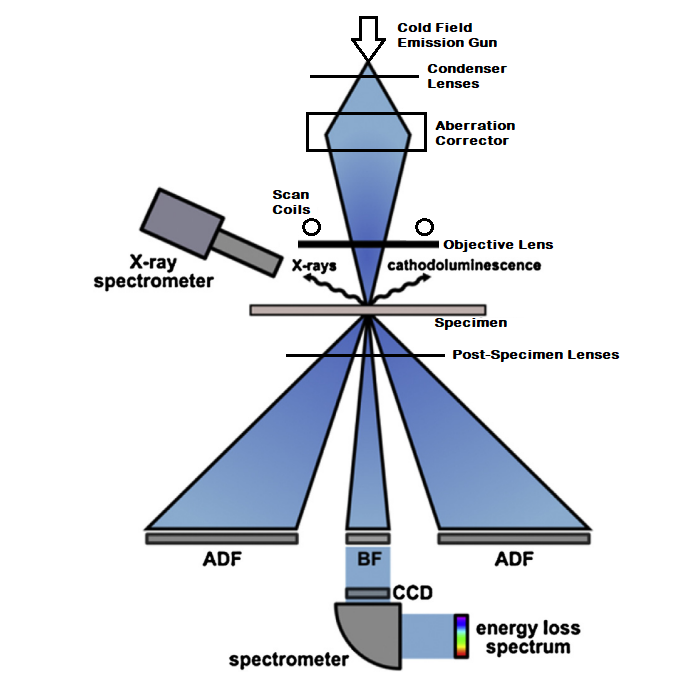
\includegraphics[width=0.75\textwidth]{fig/Fig1.png}
    \caption{Esquema que muestra los componentes principales del STEM, adaptado de la referencia \cite{foto_intro} añadiendo información suplementaria sobre ciertos instrumentos \cite{maria}.}
    \label{fig:1}
\end{figure}

En la \autoref{fig:1} se muestra el esquema de un STEM de alta resolución. El haz de electrones es generado aplicando una diferencia de potencial de decenas o centenas de kV sobre una fina punta que históricamente siempre ha estado compuesta por tungsteno, aunque actualmente se han empezado a investigar nuevos cátodos de grafeno-níquel \cite{e_gun}. Dichos electrones logran superar la barrera de potencial por efecto túnel y posteriormente atraviesan una serie de lentes capaces de corregir el haz aplicando campos magnéticos (bipolares o multipolares) que pueden llegar al orden de varios teslas.\\

Una vez el haz de electrones alcanza la muestra, se pueden producir dispersiones tanto elásticas (curvatura de la trayectoria) como inelásticas (pérdida de energía cinética). Es entonces cuando entran en juego los detectores, que comúnmente podrán suministrarnos diversas señales:

\begin{itemize}
    \item Los detectores HA (\textit{High Angle})  medirán el \textbf{ADF} (\textit{Annular Dark-Field}). Contarán en cada píxel la cantidad de electrones transmitidos que, tras atravesar la muestra, se han desviado mucho respecto al eje normal al plano de incidencia. Aquí juegan un papel protagonista los núcleos pesados, pues son capaces de interactuar fuertemente con los electrones.

    \item Para ángulos más pequeños tenemos el detector de \textbf{BF} (\textit{Bright-Field}), que mediante mínimos en el patrón de difracción es capaz de localizar las columnas atómicas menos pesadas.
    
    \item Cuando los electrones se dispersan de forma inelástica pierden una cantidad de energía que puede ser medida por \textbf{EELS} (\textit{Electron Energy Loss Spectroscopy}) mediante una CCD (\textit{Charge-Coupled Device}) o una matriz de fotodiodos.
    
    \item Cubriendo la entrada al espectrómetro se puede situar una CCD removible capaz de medir el \textbf{patrón de difracción} completo que se genera en cada punto.
    
    \item Por separado, un espectrómetro es capaz de detectar las \textbf{emisiones de rayos X} generadas por las excitaciones de electrones en la muestra.
\end{itemize}

\vspace{0.1cm}

\begin{figure}[h!]
    \centering
    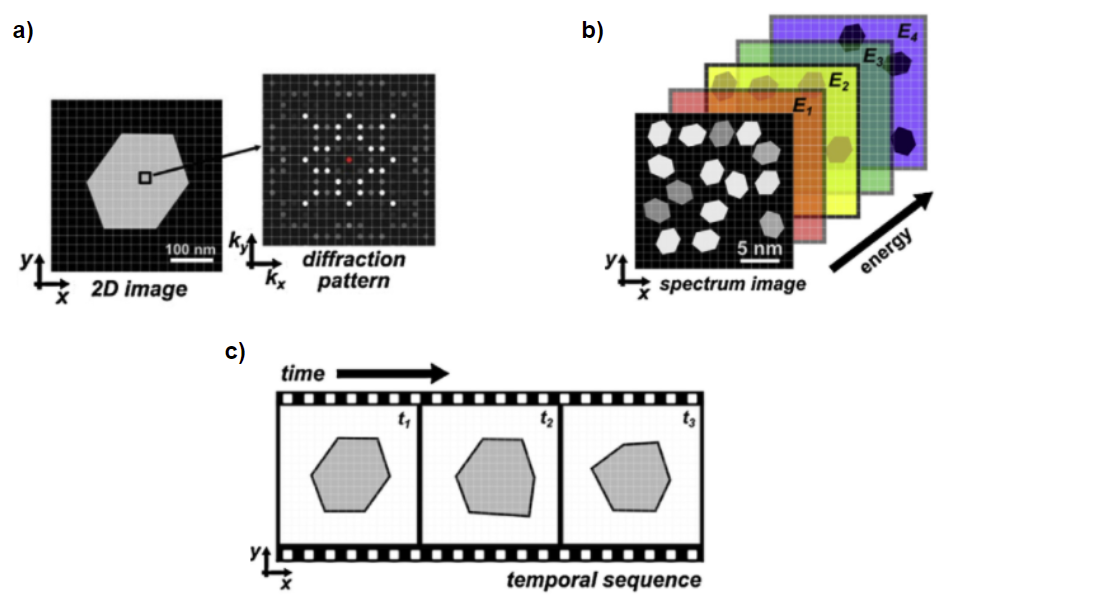
\includegraphics[width=0.9\textwidth]{fig/Fig2.png}
    \caption{En esta figura se muestra esquemáticamente todas las dimensiones en las que se puede trabajar con STEM: \textbf{a)} Espacio real-recíproco con ADF y difracción, \textbf{b)} energía mediante EELS y/o rayos X, \textbf{c)} temporal si se requiere observar la evolución de un fenómeno. Imagen adaptada de la referencia \cite{foto_intro} realizando una selección de imágenes.}
    \label{fig:2}
\end{figure}

Por esta razón, tal y como se muestra en la \autoref{fig:2}, el STEM puede aportar en una única medida datos en el dominio temporal que pueden vivir simultáneamente dentro del espacio real, recíproco y de energías. Definitivamente, contamos una gran cantidad de información que, debido a su alta dimensionalidad, plantea un escenario en el que resulta necesaria la introducción de nuevos métodos estadísticos avanzados de big data y algoritmos punteros de inteligencia artificial (IA).\\

% Párrafo siguiente añadido recientemente para indicar el enfoque principal del trabajo.

En este trabajo nos centraremos principalmente en el 4D-STEM, donde encontraremos imágenes ADF y patrones de difracción. Ambos grupos de datos en conjunto serán los que nos aporten la información necesaria para identificar y cuantificar algunos de los defectos presentes en una red cristalina.\\

% Objetivos -
\section*{Objetivos}
\addcontentsline{toc}{section}{Objetivos} \normalsize

\begin{itemize}
    \item Estudiar la relevancia de la inteligencia artificial y algunas herramientas estadísticas para el tratamiento de datos dentro del campo de la microscopía electrónica. % Cumplido
    
    \item Obtener información física relevante de un sistema en base a una serie de datos multidimensionales difícilmente interpretables. % Estamos en ello (4)
    
    \item Diseñar una red neuronal capaz de clasificar las columnas atómicas presentes en imágenes ADF. % Cumplido 
    
    \item Construir una red neuronal que ayude a detectar defectos puntuales reduciendo el ruido en imágenes 4D-STEM. % Cumplido 
    
    \item Localizar las columnas atómicas y etiquetarlas en función de su información característica. % Cumplido
    
    \item Manipular los datos experimentales mediante métodos estadísticos diseñados para reducir la dimensionalidad de un sistema. % Cumplido
    
    \item Explorar herramientas de compresión para optimizar el tamaño en memoria de las imágenes tomadas por STEM. % Cumplido
\end{itemize}